% !TEX TS-program = xelatex
% !TEX encoding = UTF-8 Unicode

% \documentclass[AutoFakeBold]{LZUThesis}
\documentclass[AutoFakeBold]{LZUThesis}
\CTEXsetup[name={第,部分}]{chapter}
% \usepackage{listings}
% \usepackage{xcolor}
% \lstset{
%     language = MATLAB,
%     identifierstyle = ,
%     basicstyle = \ttfamily,
%     stringstyle = \ttfamily,
%     showstringspaces = false,
%     % frame = shaowbox,
%     captionpos = b
% }

\lstset{
language = MATLAB,
%   backgroundcolor=\color{white},   % choose the background color; you must add \usepackage{color} or \usepackage{xcolor}  
%   basicstyle=\footnotesize,        % the size of the fonts that are used for the code  
%   breakatwhitespace=false,         % sets if automatic breaks should only happen at whitespace  
%   breaklines=true,                 % sets automatic line breaking  
%   captionpos=bl,                    % sets the caption-position to bottom  
%   commentstyle=\color{mygreen},    % comment style  
%   deletekeywords={...},            % if you want to delete keywords from the given language  
%   escapeinside={\%*}{*)},          % if you want to add LaTeX within your code  
%   extendedchars=true,              % lets you use non-ASCII characters; for 8-bits encodings only, does not work with UTF-8  
frame=shadowbox,                    % adds a frame around the code  
%   keepspaces=true,                 % keeps spaces in text, useful for keeping indentation of code (possibly needs columns=flexible)  
%   keywordstyle=\color{blue},       % keyword style  
%   %language=Python,                 % the language of the code  
%   morekeywords={*,...},            % if you want to add more keywords to the set  
numbers=none,                    % where to put the line-numbers; possible values are (none, left, right)  
%   numbersep=5pt,                   % how far the line-numbers are from the code  
%   numberstyle=\tiny\color{mygray}, % the style that is used for the line-numbers  
%   rulecolor=\color{black},         % if not set, the frame-color may be changed on line-breaks within not-black text (e.g. comments (green here))  
%   showspaces=false,                % show spaces everywhere adding particular underscores; it overrides 'showstringspaces'  
%   showstringspaces=false,          % underline spaces within strings only  
%   showtabs=false,                  % show tabs within strings adding particular underscores  
%   stepnumber=1,                    % the step between two line-numbers. If it's 1, each line will be numbered  
%   stringstyle=\color{orange},     % string literal style  
%   tabsize=2,                       % sets default tabsize to 2 spaces  
%title=myPython.py                   % show the filename of files included with \lstinputlisting; also try caption instead of title  
}  





\begin{document}
%=====%
%
%封皮页填写内容
%
%=====%

% 标题样式 使用 \title{{}}; 使用时必须保证至少两个外侧括号
%  如: 短标题 \title{{第一行}},  
% 	      长标题 \title{{第一行}{第二行}}
%             超长标题\tiitle{{第一行}{...}{第N行}}

\title{{基于MATLAB\;R2021a的简单数值计算器}}



% 标题样式 使用 \entitle{{}}; 使用时必须保证至少两个外侧括号
%  如: 短标题 \entitle{{First row}},  
% 	      长标题 \entitle{{First row}{ Second row}}
%             超长标题\entitle{{First row}{...}{ Next N row}}
% 注意:  英文标题多行时 需要在开头加个空格 防止摘要标题处英语单词粘连。

\author{\CJKfontspec{楷体}许忞欢}
\major{电子信息基地班}
\college{320200910141}
\grade{2020级}



\maketitle
\frontmatter



%中文摘要
\ZhAbstract{
    当手边没有一个很便捷且精准的方式进行数值计算时,使用一个
    基于数学语言的计算机表达编写的简单科学计算器是一个比较好的选择。
    不同于MATLAB的专业性的语言,此计算器中涉及到的各种语法取自
    初高中使用的计算器,让人感到有些亲切。}
{MATLAB, 计算器, 简约, 用户图形界面}


%英文摘要
\EnAbstract{When you don't have a convenient and precise way to do numerical
    calculations at hand, use one
    A simple scientific calculator written based on computer expression in
    mathematical language is a better choice.
    Different from the professional language of MATLAB, the calculator involved
    in the various syntax from
    Calculators used in middle and high schools make people
    feel a little friendly.  \fontspec{Times New Roman}}
{MATLAB, Calculators, Simple, GUI}

%生成目录
\tableofcontents
\thispagestyle{empty}


%文章主体
\mainmatter
\chapter{开发工具}

MATLAB是美国MathWorks公司出品的商业数学软件,
用于数据分析、无线通信、深度学习、图像处理与计算机视觉、信号处理、量化金融与风险管理、机器人,控制系统等领域。
MATLAB是matrix$\&$laboratory两个词的组合,意为矩阵工厂(矩阵实验室),
软件主要面对科学计算、可视化以及交互式程序设计的高科技计算环境。它将数值分析、矩阵计算、科学数据可视化
以及非线性动态系统的建模和仿真等诸多强大功能集成在一个易于使用的视窗环境中,为科学研究、工程设计
以及必须进行有效数值计算的众多科学领域提供了一种全面的解决方案,
并在很大程度上摆脱了传统非交互式程序设计语言(如C、Fortran)的编辑模式。

其优点如下:
\begin{enumerate}
    \item 具有完备的图形处理功能,实现计算结果和编程的可视化;
    \item 友好的用户界面及接近数学表达式的自然化语言;
    \item 功能丰富的工具箱,为用户提供了大量方便实用的处理工具。
\end{enumerate}

\chapter{程序概要分析}

\section{前期分析}
\subsection{需求分析}
面对日常生活的一些整数运算,作业中的长段的多项式运算,可能人们一般会使用掌上计算器
来解决。但是总有一些时候,在电脑面前想要做数值运算,计算器却在书包里,这时就需要一个
界面简单,语法偏向熟悉的计算器的运算工具。
\subsection{可行性分析}
MATLAB依靠其强大的功能,能够轻易地实现GUI的编写和简单的数值运算。此外,合理运用MATLAB中
集成的各种字符串函数可以更好地处理用户的输入。
\newpage
\section{程序设计思路}
\begin{figure}[htbp]
    \centering
    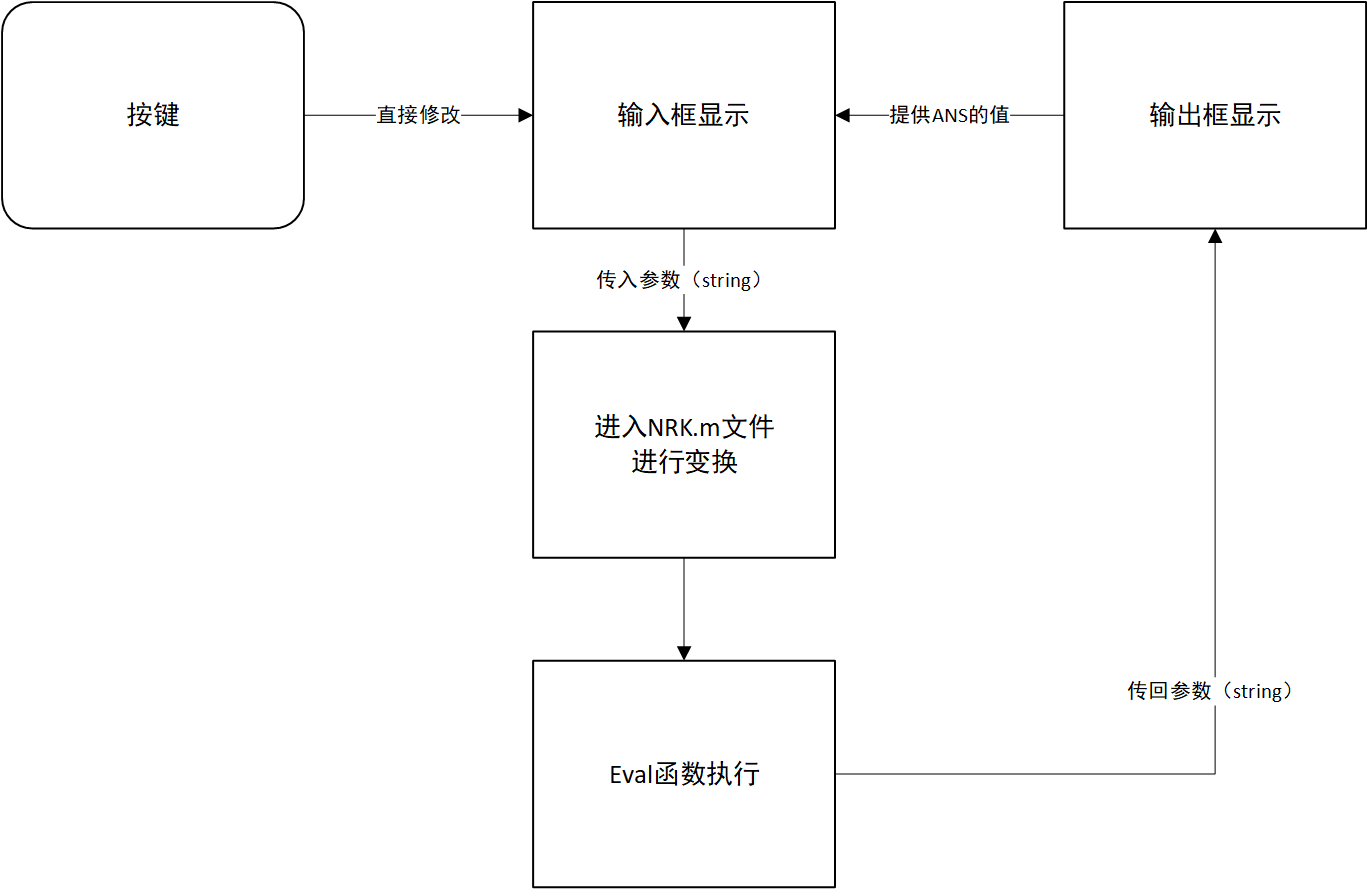
\includegraphics[keepaspectratio,width=400pt]{./figures/flow.png}
\end{figure}



%论文后部


\chapter{程序详细介绍}

\section{程序使用}
计算器布局为数字和运算符的简单面板,一共是28个按键,每按一个按键就会在输入处出现一个
符号或数字。Backspace按键可以在文本框中删去一个字符。最后按下“=”按键,程序会开始计算
并在输出文本框中出现最后的结果。这时,按下“C”按钮清空输入框,而“AC”按钮会清空输入和输出
文本框两者。其中“ANS”按钮会调用上次计算后的结果,如果使用“AC”清空则“ANS”会被重置为零。

\section{功能实现}

功能的实现分为一下几个步骤:
\begin{enumerate}
    \item 获得原始字符串
    \item 字符串处理
    \item 从字符串到计算结果及"ANS"的功能实现
\end{enumerate}

\subsection{获得原始字符串}
首先,用户按下每一个按键,都会触发那个按键的回调函数,
其中"pi"按键的回调函数如下所示。
% \newpage
\begin{lstlisting}
function Bt_piButtonPushed(app, event)
    app.input.Value = strcat(app.input.Value,'pi');
end
\end{lstlisting}

在回调函数中,我们看到名为"input"的文本框被添加了"pi"这样的 一个字符串。
在用户输入结束后,我们会在app.input.Value这个变量中看到需要计算的原始字符串。

\subsection{字符串处理}

字符串中含有$\mathrm{MATLAB}$语法中不规范的地方,在$\mathrm{NRK.m}$文件中有对此进行替换与补充的
代码如下。

\newpage

\begin{lstlisting}
    e = exp(1);
    str = replace(str,'ln(','(1/log(e))*log(');
    str = replace(str,'log3(','(1/log(3))*log(');
    str = replace(str,'log4(','(1/log(4))*log(');
    str = replace(str,'log5(','(1/log(5))*log(');
    str = replace(str,'log6(','(1/log(6))*log(');
    str = replace(str,'log7(','(1/log(7))*log(');
    str = replace(str,'log8(','(1/log(8))*log(');
    str = replace(str,'log9(','(1/log(9))*log(');
    str = replace(str,'log(','(1/log(10))*log(');
\end{lstlisting}

通过这样的替换,我们可以得到$\mathrm{MATLAB}$可以直接运行的代码。

\subsection{从字符串到计算结果及"ANS"的功能实现}

请看下一页的代码

\newpage
\begin{lstlisting}
    %% Button pushed function: Bt_cal
        function Bt_calButtonPushed(app, event)
            if isempty(app.output.Value) == 0
                app.output.Value = NRK(app.input.Value, str2double(app.output.Value));
            else
                app.output.Value = NRK(app.input.Value,0);
            end
        end
\end{lstlisting}

其中,计算功能是基于eval函数进行的.

\begin{lstlisting}
    %%NRK.m
    function str_ans = NRK(str_raw,last)
        ANS = last;
        str = str_raw;
        ……
        % 上一部分的代码已省略
        ……
        Ans = eval(str);
        str_ans = num2str(Ans);
    end
\end{lstlisting}

而ANS接受的是从输出的output文本框获得的上一次的结果值。
这实现了保留上次计算的结果可获得,即"ANS"按钮的功能。


\backmatter
\chapter{结语}
本文通过$\mathrm{MATLAB}$成功实现了简单数值计算器,并且通过简明易用的GUI提供了
使用的接口,符合原来的需求分析,也达到了可行性分析时提出的要求,达成了最初的目标。


%=======%
%引入参考文献文件
%=======%
% \bibdatabase{bib/database}%bib文件名称 仅修改bib/ 后部分
% \printbib
% \nocite{*} %显示数据库中有的,但是正文没有引用的文献


% \Appendix


% 这里是附录页,可要可不要

% \Thanks。

\end{document}